\documentclass[10pt]{article}

\usepackage[utf8]{inputenc}
\usepackage[english, russian]{babel}
\usepackage[OT1]{fontenc}

\usepackage{amsmath}
\usepackage{amsfonts}

\usepackage[
	a5paper,
	left 	=	1.5	cm,
	right 	=	1.5	cm,
	top		=	1.5	cm,
	bottom 	= 	1.5	cm
]{geometry}

\usepackage{lipsum}

\author{}
\date{}

\usepackage{graphicx}
\usepackage{subcaption}
\usepackage		[compatibility=false,
					margin		= 10	pt,
					font		= footnotesize, 
					labelfont	= bf, 
					labelsep	= endash, 
					labelfont	= bf,
					textfont	= sl,
					margin		= 0 	pt,  
					aboveskip 	= 4		pt, 
					belowskip 	= -6	pt]	{caption}
					
\usepackage{wrapfig}	
		

\begin{document}
	\begin{figure}
			    \centering
			    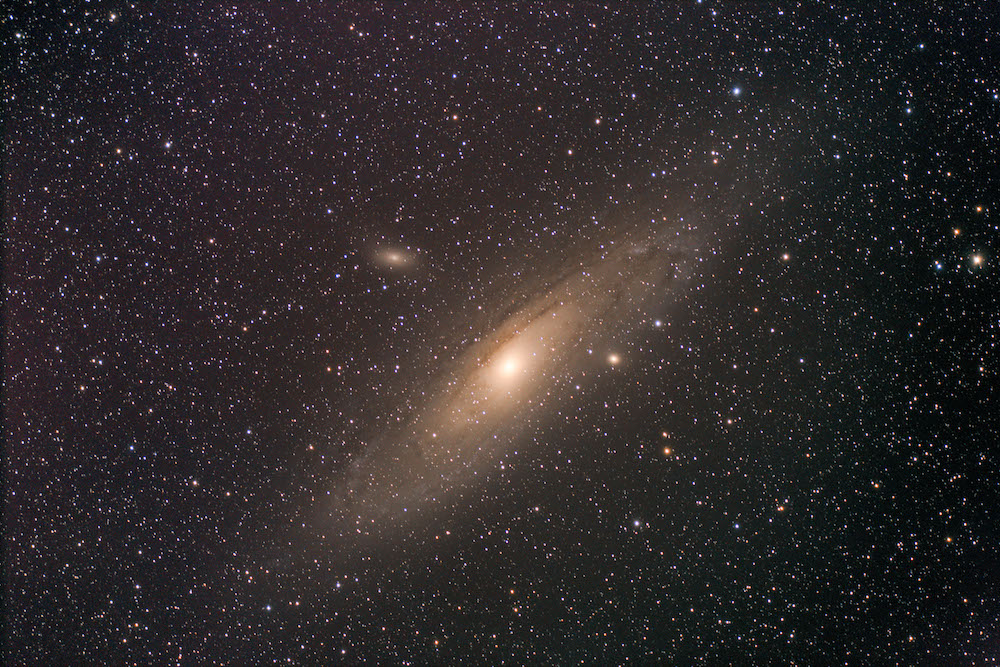
\includegraphics[width = 0.4\textwidth]{img/galaxy}
			\caption{Галактика Туманность Андромеды}
			\end{figure}
	
	\begin{figure}
				\centering
				\begin{subfigure}[b]{0.3\textwidth}
					\centering
					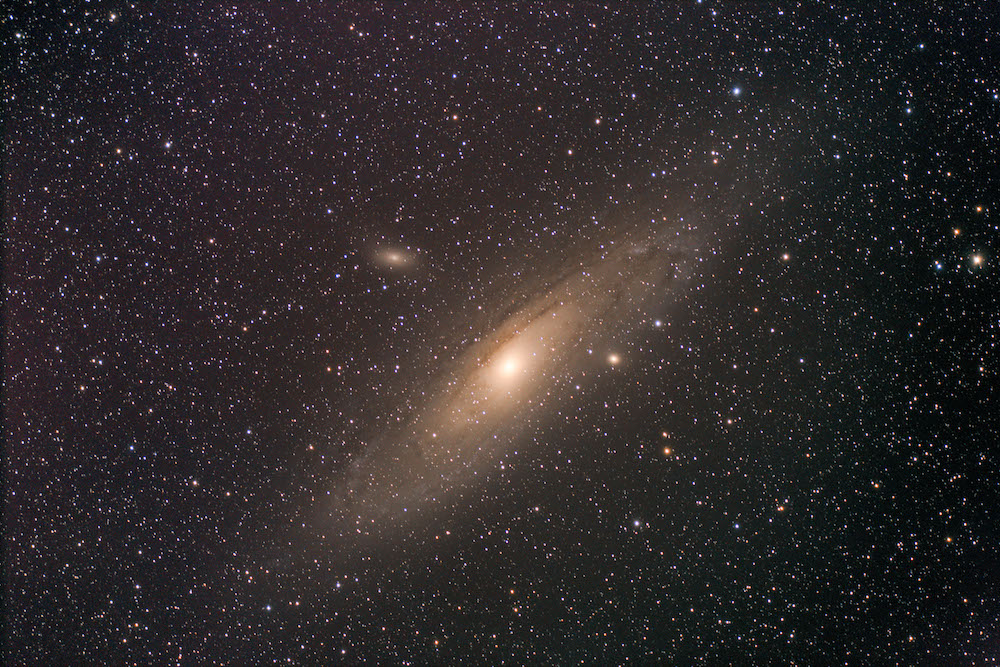
\includegraphics[width = \textwidth]{img/galaxy}
					\caption{}
				\end{subfigure}
				\begin{subfigure}[b]{0.3\textwidth}
					\centering
					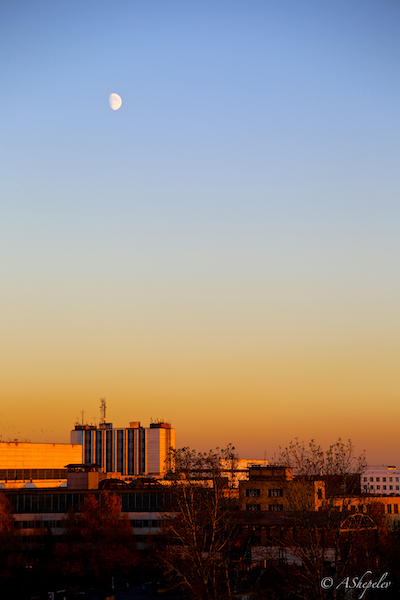
\includegraphics[width = \textwidth]{img/moon}
					\caption{}
				\end{subfigure}
				\begin{subfigure}[b]{0.3\textwidth}
					\centering
					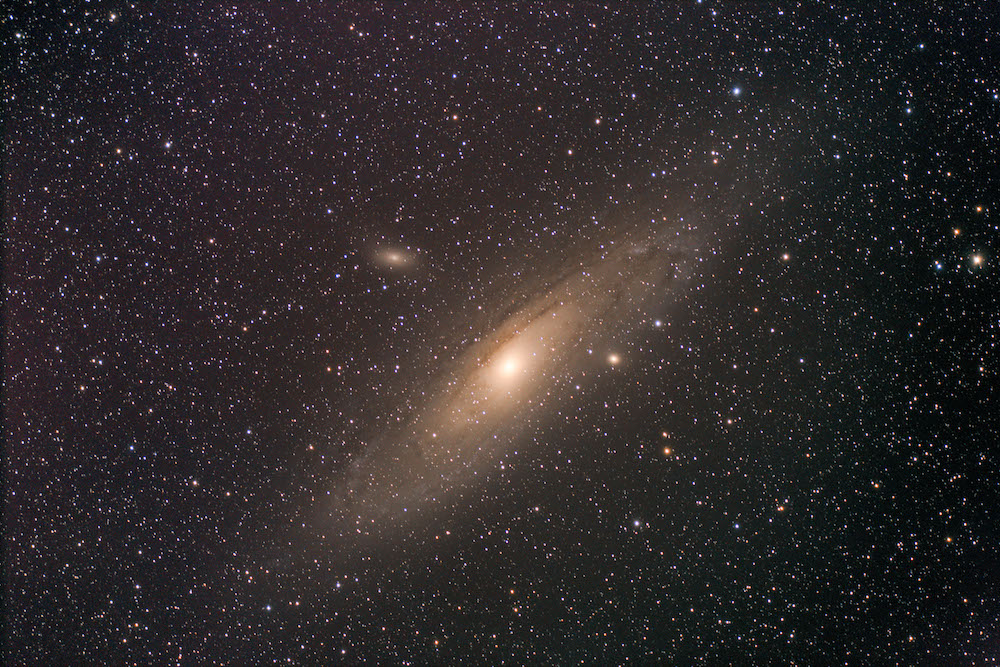
\includegraphics[width = \textwidth]{img/galaxy}
					\caption{}
				\end{subfigure}
				\caption{Фотографии}
			\end{figure}	
			
	\newpage	
	\lipsum[1-4] 
	
	\begin{wrapfigure}[18]{r}[1cm]{0.4\textwidth}
		\vspace{-1pc}
		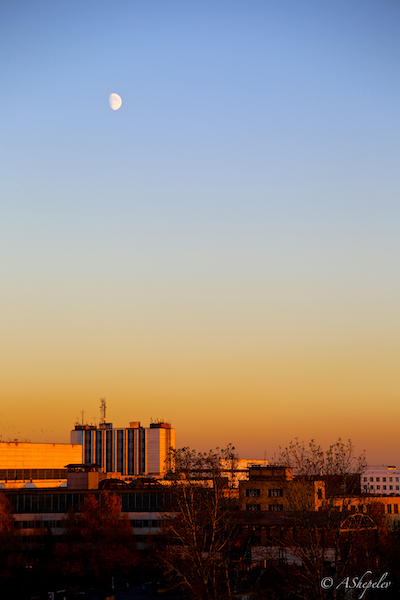
\includegraphics[width = 0.4\textwidth]{img/moon}
		\caption{}	
	\end{wrapfigure} 
	\lipsum[4-5]
	\vspace{1cm}
	
	
	\lipsum[1]
	
	\noindent
	\begin{minipage}[c][10cm][c]{0.54\textwidth}
		\lipsum[3]
	\end{minipage}
	\hfill
	\begin{minipage}[c][8cm][c]{0.44\textwidth}
		\centering
		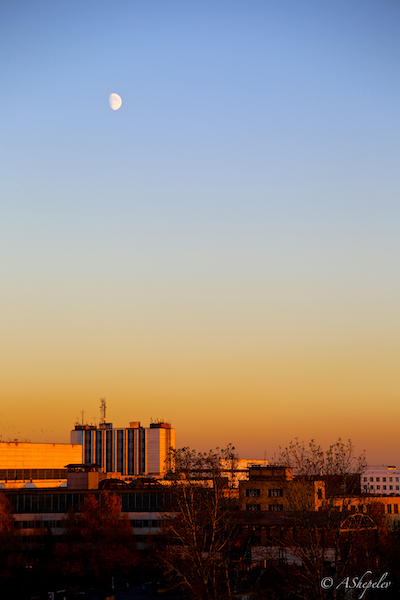
\includegraphics[width = 0.85\textwidth]{img/moon}
		\captionof{figure}{}
	\end{minipage}
	
	\lipsum[2]

\end{document}